\section{Les transformations naturelles}
Nous venons de voir la notion de foncteur, qui peuvent être vus comme
des transformations entre les catégories. Pour continuer dans la même
direction, nous allons maintenant considérer ce que sont les transformations
entre foncteurs. Ces transformations portent le nom de transformations
naturelles et jouent un rôle fondamental en théorie des catégories.

\begin{définition}[Transformation naturelle]
    Soit $\C$ et $\D$ deux catégories. Une transformation naturelle
    $\eta : F \to G$ entre deux foncteurs $F : \C \to \D$ et $G : \C \to \D$
    est une famille de flèches qui à chaque objet $X \in \ob(\C)$ associe une
    flèche $\eta_X : F(X) \to G(X) \in \hom(\D)$ telle que pour tout objet
    $Y \in \ob(\C)$ et toute flèche $f : X \to Y \in \hom(\C)$, on a
    \[
        \eta_Y \circ F(f) = G(f) \circ \eta_X
    \]
\end{définition}

Le fait que $\eta$ soit une famille de flèches plutôt qu'une application
peut sembler un peu déconcertant. Il suffit alors de se rappeler qu'une
famille indexée n'est en fait qu'une fonction sous le couvert. Ainsi, on
aurait aussi pu voir $\eta$ comme une application $\eta : \ob(\C) \to \hom(\D)$
qui à chaque objet $X \in \ob(\C)$ associe une flèche
$\eta(X) : F(X) \to G(X) \in \hom(\D)$. On préfère ici la notation indexée
parce qu'elle est plus commune dans la littérature et qu'elle nous évite
certaines difficultés de notation un peu plus loin.

Assurons-nous maintenant que l'égalité $\eta_Y \circ F(f) = G(f) \circ \eta_X$
fait bien du sens. Du côté gauche, on a que $\eta_Y : F(Y) \to G(Y)$ est une
flèche de $\D$ et que $F(f) : F(X) \to F(Y)$ est aussi une flèche de $\D$.
Ainsi, la composition de ces deux flèches fait du sens et nous donne une flèche
$\eta_Y \circ F(f) : F(X) \to G(Y)$ de $\D$. Du côté droit, on a que
$G(f) : G(X) \to G(Y)$ est une flèche de $\D$ et que $\eta_X : F(X) \to G(X)$
est aussi une flèche de $\D$. Ainsi, la composition de ces deux flèches fait
du sens et nous donne une flèche $G(f) \circ \eta_X : F(X) \to G(Y)$ de $\D$.
Si elle n'est pas très intuitive, l'égalité de ces deux expressions fait donc
au moins du sens.

Or, il existe une manière visuelle de se représenter cette équation qui nous
aidera à en tirer un peu d'intuition. Il suffit de représenter les catégories
$\C$ et $\D$ ainsi que l'action de $F$, $G$ et $\eta$ sur deux objets
quelconques $X,Y \in \ob(\C)$ et une flèche $f : X \to Y$.

\[
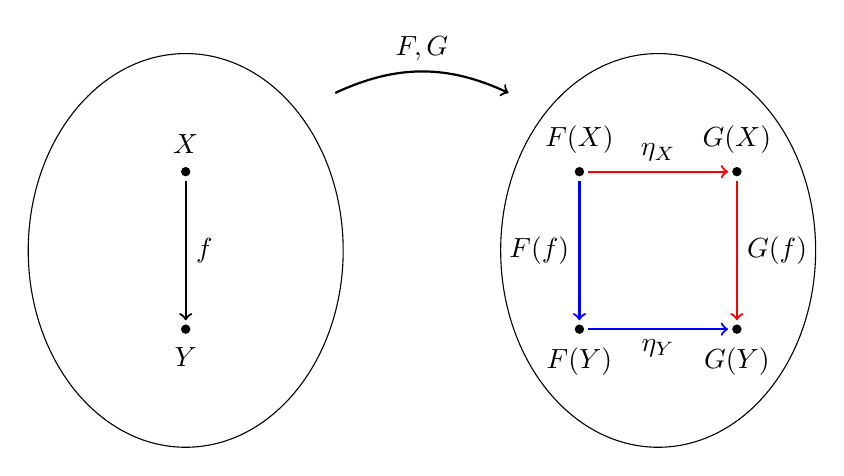
\begin{tikzpicture}
    % Catégorie C
    \draw (2,2) ellipse (2cm and 2.5cm);
    \node(C) at (3,4.6) {$\C$};

    \draw (2,3) node[circle, inner sep=1.2pt, outer sep=1.5pt, fill=black, label={above:{$X$}}] (X) {};
    \draw (2,1) node[circle, inner sep=1.2pt, outer sep=1.5pt, fill=black, label={below:{$Y$}}] (Y) {};
    \draw [thick, ->] (X) -- node[right] {$f$} (Y);

    % Catégorie D
    \draw (8,2) ellipse (2cm and 2.5cm);
    \node(D) at (9,4.6) {$\D$};
    \draw (7,3) node[circle, inner sep=1.2pt, outer sep=1.5pt, fill=black, label={above:{$F(X)$}}] (FX) {};
    \draw (7,1) node[circle, inner sep=1.2pt, outer sep=1.5pt, fill=black, label={below:{$F(Y)$}}] (FY) {};
    \draw [blue, thick, ->] (FX) -- node[color=black, left] {$F(f)$} (FY);

    \draw (9,3) node[circle, inner sep=1.2pt, outer sep=1.5pt, fill=black, label={above:{$G(X)$}}] (GX) {};
    \draw (9,1) node[circle, inner sep=1.2pt, outer sep=1.5pt, fill=black, label={below:{$G(Y)$}}] (GY) {};
    \draw [red, thick, ->] (GX) -- node[color=black, right] {$G(f)$} (GY);

    % Foncteurs
    \draw [thick, ->] (3.9,4) to [bend left=25] node[above] {$F,G$} (6.1,4);

    % Transformation naturelle
    \draw [red, thick, ->] (FX) -- node[color=black, above] {$\eta_X$} (GX);
    \draw [blue, thick, ->] (FY) -- node[color=black, below] {$\eta_Y$} (GY);
\end{tikzpicture}
\]

L'équation $\eta_Y \, \circ F(f) = G(f) \circ \, \eta_X$ peut se lire comme
``$\eta_Y$ après $F(f)$ doit être égal à $G(f)$ après $\eta_X$'', ce
qui veut simplement dire que les chemins bleus et rouges doivent en fait
donner le même résultat, et ce peut importe les $X$, $Y$ et $f$ considérés.
Ainsi, l'équation présentée plus haut peut se réécrire sous une forme plus
visuelle en affirmant que le diagramme suivant commute:
\[
\begin{tikzcd}
    F(X) \arrow[d, blue, "F(f)"' black] \arrow[r, red, "\eta_X" black] & G(X) \arrow[d, red, "G(f)" black] \\
    F(Y) \arrow[r, blue, "\eta_Y" black] & G(Y)
\end{tikzcd}
\]


%%%%%%%%%%%%%%%%%%%%%%%%%%%%%%%%%%%%%%%%%%%%%%%%%%%%%%%%%%%%%%%%%%%%%%%%%%%%%%
\subsection{Les transformations naturelles dans Hana}
Dans Hana, un foncteur est un type généralisé paramétré et une flèche
$f : X \to Y$ est une fonction d'un type généralisé \icpp{X} vers un type
généralisé \icpp{Y}. Ainsi, étant donné deux types généralisés paramétrés
\icpp{F} et \icpp{G} qui sont des foncteurs, une transformation naturelle
$\icpp{nat} : \icpp{F} \to \icpp{G}$ sera une famille de fonctions qui à
chaque type généralisé \icpp{X} associe une fonction
$\icpp{nat<X>} : \icpp{F(X)} \to \icpp{G(X)}$. De plus, la loi
énoncée plus haut se traduit dans le langage de Hana en disant que pour tout
type généralisé \icpp{Y} et toute fonction $\icpp{f} : \icpp{X} \to \icpp{Y}$,
on doit avoir
\begin{cpp}
    compose(nat<Y>, transform(-, f)) == compose(transform(-, f), nat<X>)
\end{cpp}

Par exemple, essayons d'écrire une fonction qui serait une transformation
naturelle du foncteur \icpp{Maybe} vers le foncteur \icpp{Tuple}. On cherche
donc une famille de fonctions qui à chaque type généralisé \icpp{X} associe
une fonction $\icpp{toTuple<X>} : \icpp{Maybe(X)} \to \icpp{Tuple(X)}$. La
définition la plus évidente d'une telle fonction serait
\begin{align*}
    \icpp{toTuple<X>} : \icpp{Maybe(X)} &\to \icpp{Tuple(X)} \\
                        \icpp{just(x)} &\mapsto \icpp{make_tuple(x)} \\
                        \icpp{nothing} &\mapsto \icpp{make_tuple()}
\end{align*}

ce qui se traduit dans Hana par
\begin{cpp}
    template <typename X, typename T>
    auto toTuple(_just<T> j) {
        return make_tuple(from_just(j));
    }

    template <typename X>
    auto toTuple(_nothing) {
        return make_tuple();
    }
\end{cpp}

A-t-on vraiment une transformation naturelle? Si c'est le cas, on devrait
avoir que pour tout type généralisé \icpp{Y} et toute fonction
$\icpp{f} : \icpp{X} \to \icpp{Y}$,
\begin{cpp}
    compose(toTuple<Y>, transform(-, f)) == compose(transform(-, f), toTuple<X>)
\end{cpp}

ce qui est équivalent à dire que pour tout objet \icpp{m} de type généralisé
\icpp{Maybe(X)},
\begin{cpp}
    toTuple<Y>(transform(m, f)) == transform(toTuple<X>(m), f)
\end{cpp}

Énoncé de cette manière, il est assez évident que c'est le cas. En effet, si
\icpp{m} est un \icpp{just(x)}, alors
\begin{cpp}
    toTuple<Y>(transform(just(x), f)) == toTuple<Y>(just(f(x)))
                                      == make_tuple(f(x))
                                      == transform(make_tuple(x), f)
                                      == transform(toTuple<X>(just(x)), f)
\end{cpp}

De manière similaire, si \icpp{m} est un \icpp{nothing}, alors
\begin{cpp}
    toTuple<Y>(transform(nothing, f)) == toTuple<Y>(nothing)
                                      == make_tuple()
                                      == transform(make_tuple(), f)
                                      == transform(toTuple<X>(nothing), f)
\end{cpp}

et \icpp{toTuple} est donc bien une transformation naturelle. Cependant, cette
définition n'est pas la seule qui permette à \icpp{toTuple} d'être une
transformation naturelle. En effet, on aurait aussi pu considérer
\begin{cpp}
    template <typename X, typename T>
    auto toTuple2(_just<T> j) {
        return make_tuple(from_just(j), from_just(j));
    }

    template <typename X>
    auto toTuple2(_nothing) {
        return make_tuple();
    }
\end{cpp}

Ici, la différence est que l'on crée un tuple avec deux copies du même élément
lorsqu'on a un \icpp{just(x)}. Il est facile de voir que c'est une
transformation naturelle. En effet, on a
\begin{cpp}
    toTuple2<Y>(transform(just(x), f)) == toTuple2<Y>(just(f(x)))
                                       == make_tuple(f(x), f(x))
                                       == transform(make_tuple(x, x), f)
                                       == transform(toTuple2<X>(just(x)), f)
\end{cpp}

Ceci est en fait une manifestation du résultat plus général suivant.
\begin{théorème}
    Soit $F,G,H : \C \to \D$ des foncteurs et $\alpha : F \to G$, $\beta : G \to H$
    des transformations naturelles. Alors la famille de flèches $\beta \circ \alpha$
    définie par $(\beta \circ \alpha)_X = \beta_X \circ \alpha_X$ est une
    transformation naturelle $F \to H$. En d'autres mots, la composition de
    deux transformations naturelles est une transformation naturelle.
\end{théorème}
\begin{proof}
    Soit $X, Y \in \ob(\C)$ des objets de $\C$ et $f : X \to Y \in \hom(\C)$
    une flèche de $\C$. Premièrement, $\beta_X \circ \alpha_X$ est bien une
    flèche $F(X) \to H(X)$, puisque $\alpha_X$ est une flèche $F(X) \to G(X)$
    et $\beta_X$ est une flèche $G(X) \to H(X)$. Ensuite, on a
    \begin{align*}
        (\beta \circ \alpha)_Y \circ F(f)
            &= (\beta_Y \circ \alpha_Y) \circ F(f)                          \\
            &= \beta_Y \circ (G(f) \circ \alpha_X)                          \\
            &= (H(f) \circ \beta_X) \circ \alpha_X                          \\
            &= H(f) \circ (\beta \circ \alpha)_X
    \end{align*}

    ce qui montre que $\beta \circ \alpha$ est naturelle.
\end{proof}

Dans l'exemple plus haut, \icpp{toTuple2} était simplement la composition
de la transformation naturelle \icpp{toTuple} définie plus haut avec la
transformation naturelle \icpp{twice} définie par
\begin{align*}
    \icpp{twice<X>} : \icpp{Tuple(X)} &\to \icpp{Tuple(X)} \\
                      \icpp{make_tuple(x1, ..., xn)} &\mapsto \icpp{make_tuple(x1, ..., xn, x1, ..., xn)}
\end{align*}
